\section{Illustration: Applying the Score to Ten Open Textbooks}
\label{sec:illustration}

This section applies the specification to real resources. It is an \emph{illustration}, not a validation: every score was produced by an AI agent from the same model family, and no human reviewer scored the same resources. Its purposes are to show that the instrument can be applied at low cost, to show what it surfaces, to measure how stable the scores are across two independent passes, and to expose where the specification is too loose.

\subsection{Method}
\paragraph{Selection.}
No public title-level ranking of OER popularity exists that we could find, so ``widely used'' is a judgment. We chose six OpenStax titles (College Physics 2e, Biology 2e, Psychology 2e, Principles of Economics 3e, Calculus Volume 1, Anatomy and Physiology 2e) and four titles from other publishers (OpenIntro Statistics; \emph{A First Course in Linear Algebra} by Beezer; \emph{Think Python}; \emph{Eloquent JavaScript}) to span subjects, publishers and source formats. This is a convenience sample, not a random one, and it over-represents one publisher.

\paragraph{Two passes.}
All ten titles were scored twice on 31 October 2026, by separate agents that did not see each other's scores. Each agent received an identical brief containing the ten metrics, the descriptors of Table~\ref{tab:bands}, the four scoring rules and the decision rule of Equation~\ref{eq:decision}. Agents used web search, page and API fetches and small scripts, and they ran on the default subagent model, which inherits the session's model (Claude Sonnet 5.5).
\begin{itemize}[leftmargin=*,itemsep=2pt]
  \item \emph{First pass (one chapter).} Metrics 1 to 5 were scored from front matter and the fifth chapter in the table of contents; metrics 6 to 10 from the whole work.
  \item \emph{Second pass (three chapters).} We changed the sampling after noticing that one chapter is a thin basis for the quality metrics. Metrics 1 to 5 were scored separately for the first, middle and last numbered chapters, and the reported score is the mean rounded half up. Metrics 6 to 10 were again scored from the whole work. Agents worked in their own folders.
\end{itemize}
Each agent returned a record with the scores, one or two sentences of located evidence per metric, a self-reported confidence per metric, a list of what it could not verify, a Flesch--Kincaid grade for each sampled chapter and image alternative-text counts. Unless stated otherwise, the results below are from the second pass; the first pass is used for the comparison in Section~\ref{sec:retest}.

\paragraph{Scripted census.}
Separately, we ran the 13 scripted book-level completeness checks of a companion evaluator skill \cite{oerevaluator} on MkDocs book projects in the author's workspace. The checks are static analysis of files on disk: license, creators, sponsor, objectives, learners, prerequisites, instructions, accessibility mention, technical requirements, references, internal links, practice questions and image alternative text.

\emph{How the 101 were chosen.} Selection was by file layout, not by content. The workspace has 160 top-level folders; 143 contain a \texttt{mkdocs.yml}; 111 of those also have a \texttt{docs/chapters} folder; and the 101 with at least five entries there form the census. The threshold of five was fixed before the run to skip scaffolds and stubs and was not tuned against results; a threshold of one would admit 111. Because the rule looks only at layout, the 101 are not all textbooks. They include repositories that appear from their names to be tooling, documentation or hardware projects (for example a repository of agent skills and a catalog of simulations), and they include the companion book from which the rubric comes. We did not classify them by hand; Section~\ref{sec:census} reports the effect of excluding the obvious candidates.

\emph{Which versions.} Before the run we updated every one of the 111 candidates on 31 October 2026 with \texttt{git pull --ff-only}, which fast-forwards or refuses and never merges. Of the 101 census books, 76 were already current, 6 fast-forwarded, and 19 refused: 11 have histories that diverge from their remote, 5 contain unresolved merge conflicts, and 3 have local edits that the update would overwrite. Refused books were inspected as they stand locally. The checks read the working tree, not a commit, so the 40 books with uncommitted edits were inspected with those edits. The commit, dirty state and pull outcome of every book are recorded with the data.

\subsection{Scores of ten textbooks}
Table~\ref{tab:scores} gives the second-pass results. Totals range from 60 to 81 (mean 72.9, median 77.5). Six titles meet the Adopt rule of Equation~\ref{eq:decision}, all from OpenStax; none reaches the excellent band, and the four titles from other publishers all land in Revise. Figure~\ref{fig:qr} plots Q against R, and Figure~\ref{fig:profile} shows each metric's mean and range.

\begin{table}[htbp]
\centering
\caption{OpenBook QR Scores for ten open textbooks from the three-chapter pass, sorted by total. Metric scores are $s_1$ to $s_{10}$ in the order of Table~\ref{tab:metrics}. $T_1$ is the total from the independent one-chapter pass. Scores are provisional and unvalidated: one AI-agent reviewer per title per pass.}
\label{tab:scores}
\scriptsize
\setlength{\tabcolsep}{3.0pt}
\begin{tabular}{@{}lccccccccccccccc@{}}
\toprule
Title & $s_1$ & $s_2$ & $s_3$ & $s_4$ & $s_5$ & $s_6$ & $s_7$ & $s_8$ & $s_9$ & $s_{10}$ & Q & R & T & $T_1$ & Decision \\
\midrule
OpenStax Physics 2e & 8 & 8 & 8 & 8 & 8 & 8 & 9 & 7 & 9 & 8 & 40 & 41 & 81 & 79 & Adopt \\
OpenStax Calculus 1 & 8 & 8 & 8 & 8 & 8 & 9 & 8 & 7 & 9 & 8 & 40 & 41 & 81 & 73 & Adopt \\
OpenStax Anat.\ \& Phys.\ 2e & 8 & 8 & 8 & 8 & 6 & 8 & 9 & 8 & 9 & 8 & 38 & 42 & 80 & 80 & Adopt \\
OpenStax Economics 3e & 7 & 8 & 8 & 8 & 7 & 9 & 8 & 8 & 9 & 8 & 38 & 42 & 80 & 83 & Adopt \\
OpenStax Psychology 2e & 7 & 8 & 8 & 8 & 6 & 9 & 8 & 7 & 9 & 8 & 37 & 41 & 78 & 76 & Adopt \\
OpenStax Biology 2e & 8 & 8 & 7 & 8 & 5 & 8 & 9 & 7 & 9 & 8 & 36 & 41 & 77 & 76 & Adopt \\
Think Python 3e & 8 & 5 & 8 & 5 & 6 & 7 & 8 & 4 & 10 & 6 & 32 & 35 & 67 & 69 & Revise \\
OpenIntro Statistics & 8 & 6 & 7 & 3 & 8 & 8 & 5 & 3 & 9 & 7 & 32 & 32 & 64 & 73 & Revise \\
Eloquent JavaScript 4e & 8 & 3 & 7 & 6 & 5 & 6 & 8 & 2 & 8 & 8 & 29 & 32 & 61 & 68 & Revise \\
Beezer Linear Algebra & 6 & 4 & 8 & 3 & 8 & 7 & 7 & 2 & 8 & 7 & 29 & 31 & 60 & 59 & Revise \\
\midrule
Mean (all ten) & 7.6 & 6.6 & 7.7 & 6.5 & 6.7 & 7.9 & 7.9 & 5.5 & 8.9 & 7.6 & 35.1 & 37.8 & 72.9 & 73.6 & \\
\bottomrule
\end{tabular}
\end{table}

\begin{figure}[htbp]
  \centering
  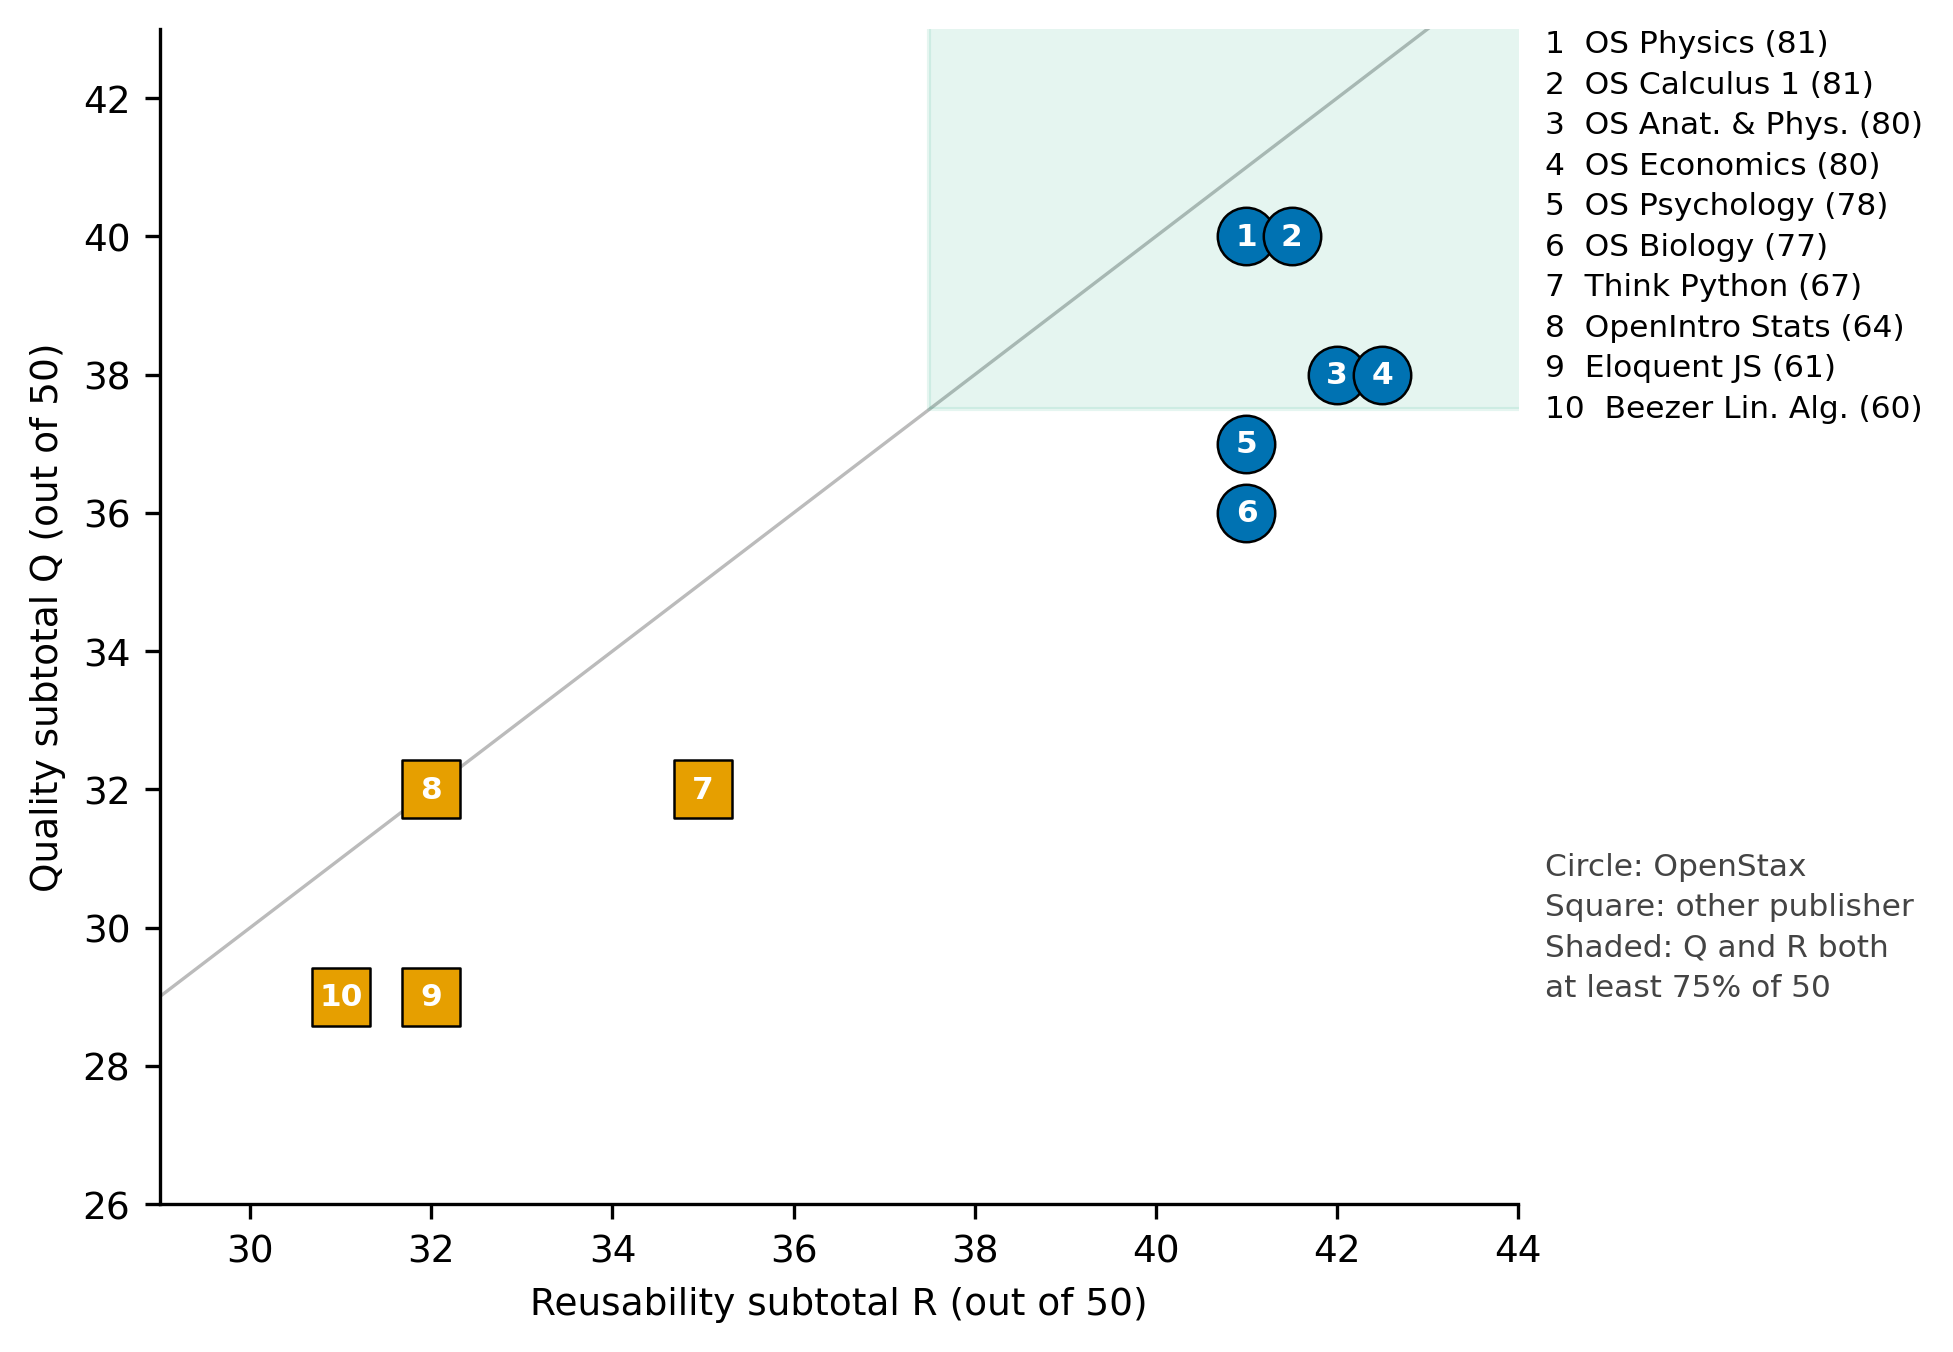
\includegraphics[width=0.92\textwidth]{figures/qr-scatter.png}
  \caption{Quality subtotal Q against reusability subtotal R for the ten scored textbooks (three-chapter pass), numbered by total score with a key at right. Every title sits on or below the diagonal, so reusability is at least as strong as quality for all ten. The four titles in the shaded region have both subtotals at least 75 percent of 50. Points with identical Q and R are offset slightly so both remain visible.}
  \label{fig:qr}
\end{figure}

\begin{figure}[htbp]
  \centering
  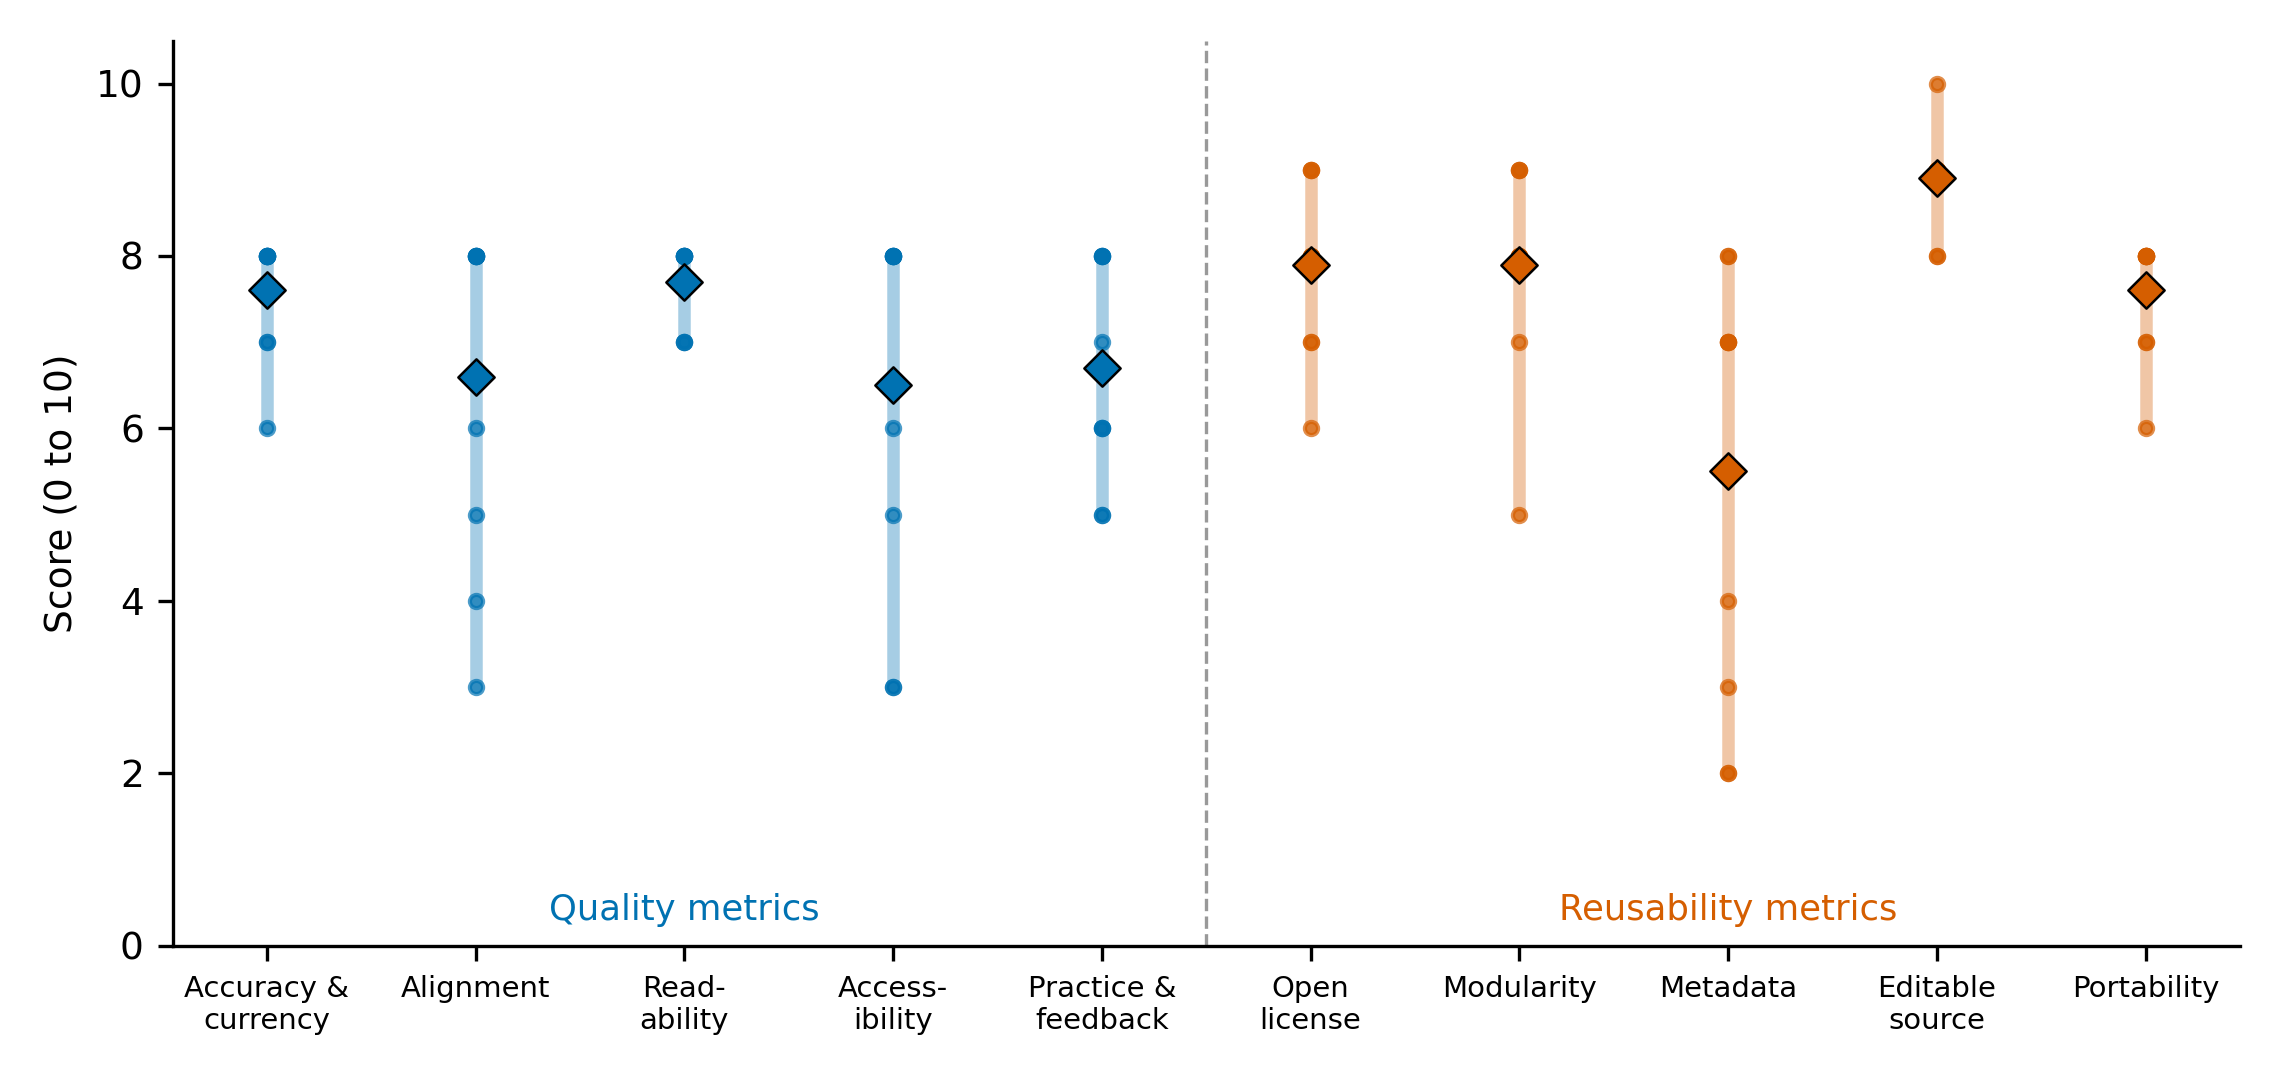
\includegraphics[width=0.95\textwidth]{figures/metric-profile.png}
  \caption{Score distribution for each of the ten metrics across the ten textbooks (three-chapter pass): individual scores (dots), range (bar) and mean (diamond), with quality metrics in blue and reusability metrics in vermilion. Metadata has the lowest mean and the widest spread among reusability metrics; accessibility and alignment have the widest spread among quality metrics.}
  \label{fig:profile}
\end{figure}

\subsection{What the scores surface}
\paragraph{Reusability is at least as strong as quality.}
In the second pass R is at least Q for all ten titles, by 0 to 5 points (mean R 37.8, mean Q 35.1). A plausible reading is that content quality is simply harder to verify from public pages than a license or a source repository, so reviewers score the quality metrics conservatively; another is that open-textbook projects invest heavily in packaging. The data cannot separate these explanations. They do show why the two halves need to be reported separately: a single total of 67 for \emph{Think Python} hides that its editable-source score is the maximum (10) while its alignment and accessibility scores are only 5 and 5.

\paragraph{Metadata is the weakest metric.}
Metadata has the lowest mean (5.5) and ranges from 2 to 8. Reviewers repeatedly found descriptive and citation tags in page source but no structured educational metadata such as subject and level, or machine-readable license fields, and they found blank metadata in the one PDF-only book. This echoes the long-standing emphasis on metadata quality in learning-object repositories \cite{ochoa2009}.

\paragraph{Editable source is the strongest.}
Editable source has the highest mean (8.9, range 8 to 10), consistent with open-textbook projects publishing source on public hosting sites. Learning-outcome alignment (mean 6.6, range 3 to 8) and accessibility (mean 6.5, range 3 to 8) show the widest spread among quality metrics. For three titles (Think Python, Eloquent JavaScript, Beezer) the reviewers found no clear per-section learning outcomes. For OpenIntro Statistics, the second-pass reviewer found that the book's ``screen-reader'' PDF is marked untagged and that no alternative text appeared in its extracted text, which the first-pass reviewer could not check.

\paragraph{Licenses: eight of ten carry a NonCommercial term, and the rubric is under-specified.}
The six OpenStax titles and \emph{Think Python} are CC BY-NC-SA 4.0, and \emph{Eloquent JavaScript} is CC BY-NC 3.0; OpenIntro is CC BY-SA 3.0 and Beezer's text is under the GNU Free Documentation License. No title is CC BY. The license metric scored 8 or 9 for the six NC-SA OpenStax titles, 7 for \emph{Think Python} (also NC-SA) and 6 for \emph{Eloquent JavaScript}. Reviewers described weighing the NonCommercial term, the license version, third-party notices and whether a license line appears on every page, and they weighed them differently; the descriptors of Table~\ref{tab:bands} do not say how a restrictive-but-clear license should be scored. This is the kind of under-specification an anchored rubric must remove (R1).

\paragraph{Agents report their own uncertainty.}
Each agent listed between 6 and 8 things it could not verify, such as whether a license notice appears on every page, whether LMS packages import cleanly, and whether alternative text is meaningful. These statements are useful, but they are self-reports and have not been checked against an independent reviewer.

\subsection{Stability across the two passes}
\label{sec:retest}
The first pass (one chapter) and second pass (three chapters) are independent applications of the same instrument by different agents of the same model family. Comparing them gives a first, rough estimate of how stable scores are; Figure~\ref{fig:passes} plots the totals.

\begin{figure}[htbp]
  \centering
  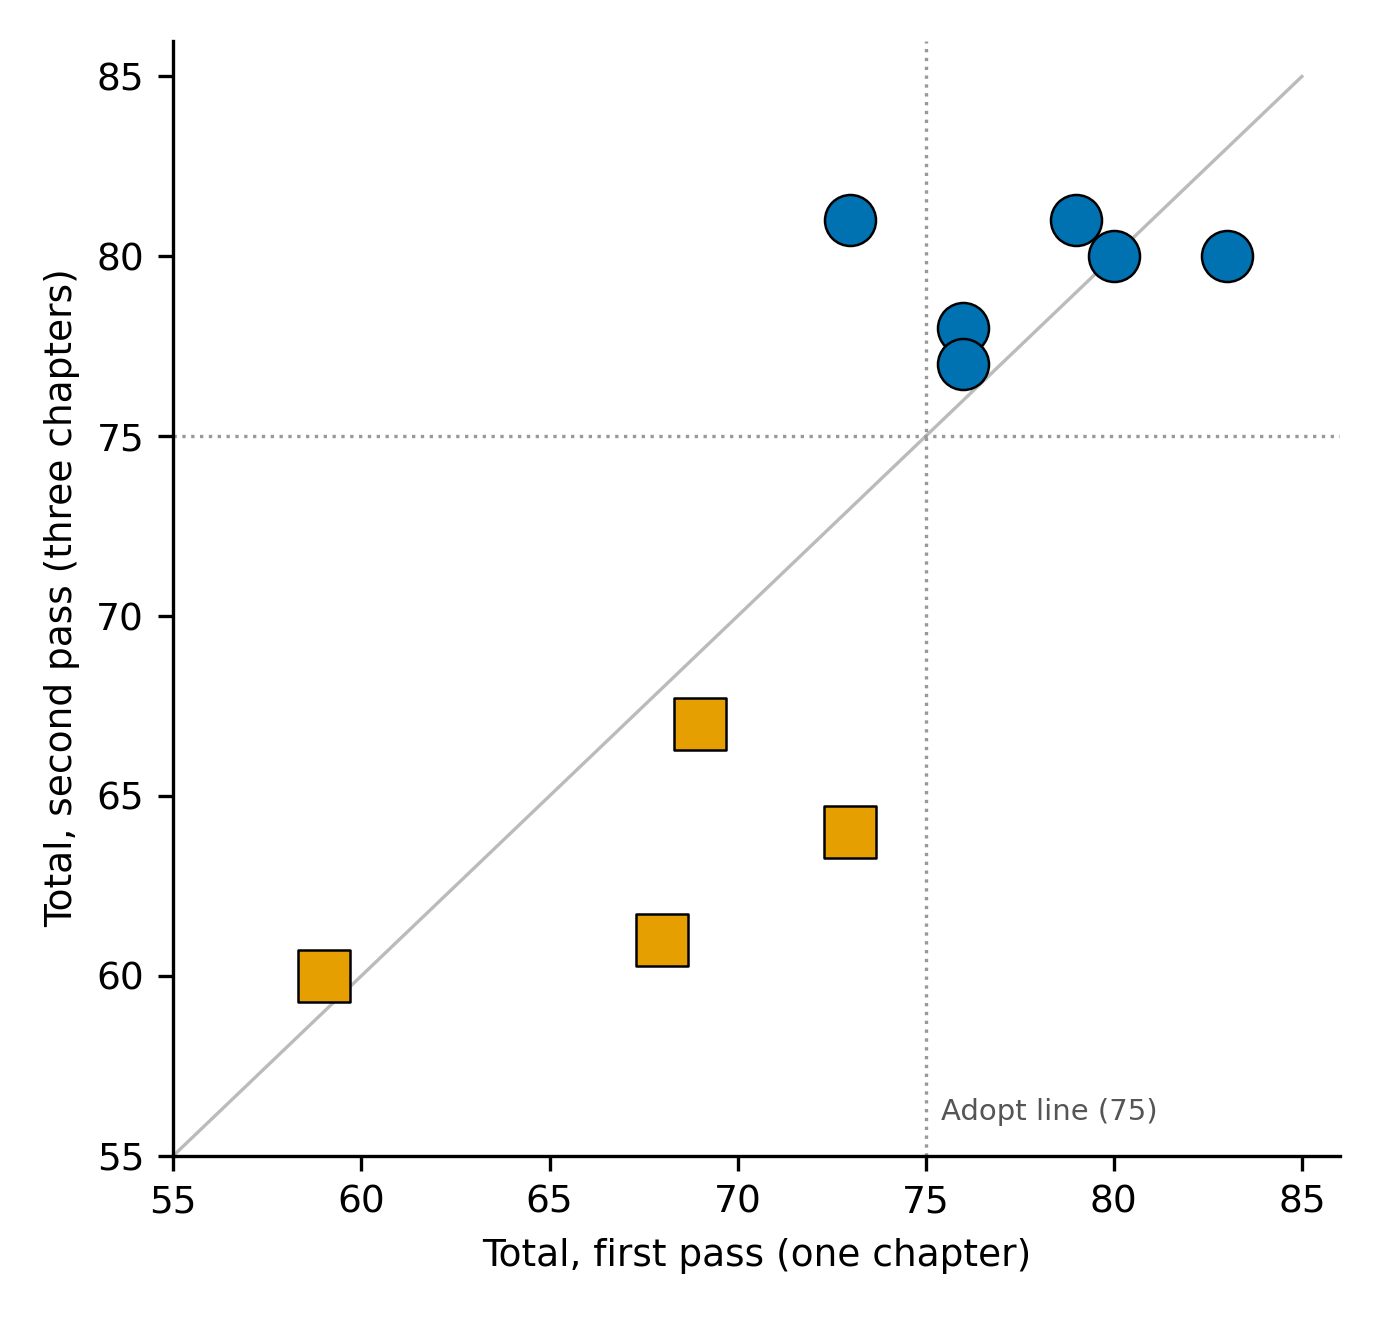
\includegraphics[width=0.62\textwidth]{figures/passes-scatter.png}
  \caption{Total score from the first, one-chapter pass (horizontal) against the second, three-chapter pass (vertical) for the ten textbooks; circles are OpenStax titles and squares are other publishers. Points near the diagonal were scored alike; the dotted lines mark the Adopt threshold of 75. One title (Calculus Volume 1) crosses the threshold between passes and the other nine keep their decision.}
  \label{fig:passes}
\end{figure}

Totals differ by a mean of 3.5 points between passes (rank correlation 0.75), and nine of the ten decisions are unchanged; Calculus Volume 1 moves from Revise (73) to Adopt (81). Across the 100 metric scores, the two passes agree exactly 46 percent of the time and within one point 88 percent of the time, with a quadratic-weighted kappa of 0.80 \cite{cohen1960,landis1977}. For the five reusability metrics, which both passes scored from the whole work, exact agreement is 44 percent, agreement within one point is 90 percent and the weighted kappa is 0.86. For the five quality metrics, where the sampled chapters also changed, the figures are 48 percent, 86 percent and 0.71.

Three caveats apply. The kappa pools all ten metrics, so it partly reflects differences between books; with ten books we cannot estimate it per metric. Both passes used the same model family and the same brief, so their errors may be correlated, and this agreement is probably an upper bound on what independent human reviewers would achieve. And because the reviewer and the sampled chapters changed together for metrics 1 to 5, the comparison cannot separate reviewer noise from chapter effects there. The reusability metrics isolate reviewer noise, and their mean absolute difference (0.66 points) is similar to that for the quality metrics (0.72), which suggests that chapter choice adds little beyond reviewer noise for most metrics. The exception is practice with feedback: it has the lowest exact agreement (2 of 10) and the largest mean difference (1.4 points), and its per-chapter scores vary the most within a book (mean range 1.3 points, up to 6). In \emph{Think Python}, the first and middle chapters score 8 while the final reflective chapter, which has no exercises, scores 2.

Chapter choice matters most where chapters differ in kind. Across the ten books the per-chapter quality subtotal (out of 50) ranged by a mean of 2.5 points between a book's best and worst sampled chapter, but by 8 for \emph{Think Python} and 6 for OpenStax College Physics, whose final chapters are short or conceptual. A one-chapter sample is therefore adequate for some books and misleading for others, and a reviewer cannot tell in advance which.

\subsection{Cost of scoring}
Table~\ref{tab:cost} reports what scoring cost. The first pass used 827{,}549 tokens and 135 tool calls and took about 2 minutes 25 seconds of wall-clock time with ten agents in parallel. The three-chapter pass used 860{,}984 tokens and 176 tool calls and took about 3 minutes 37 seconds. Per title, the second pass took a mean of about 86{,}100 tokens and 121 seconds. Together the two passes used about 1.69 million tokens. Tripling the number of sampled chapters raised tokens by only 4 percent and time per title by 28 percent, because most of an agent's effort goes to whole-work checks and to locating evidence, not to reading additional chapters. Tokens used by the main session to coordinate the agents and to draft the paper are not included.

\begin{table}[htbp]
\centering
\caption{Resource cost of scoring ten textbooks, one agent per title, all run in parallel. Token counts are the totals reported by the agent harness for each agent. Cost is for one reviewer pass and does not include any human checking.}
\label{tab:cost}
\small
\begin{tabular}{@{}llrrr@{}}
\toprule
Pass & Measure & Mean per title & Minimum & Maximum \\
\midrule
One chapter & Tokens used & 82{,}755 & 71{,}761 & 102{,}022 \\
 & Elapsed time (seconds) & 94 & 47 & 144 \\
 & Tool calls & 13.5 & 6 & 21 \\
\addlinespace
Three chapters & Tokens used & 86{,}098 & 74{,}385 & 97{,}170 \\
 & Elapsed time (seconds) & 121 & 52 & 217 \\
 & Tool calls & 17.6 & 7 & 29 \\
\bottomrule
\end{tabular}
\end{table}

No book needed to be downloaded in full: agents read pages, archives and public APIs, and the working folders they used for scripts and fetched pages held about 109 MB in total (97 MB of it in one title's folder). The 101 scripted-census reports occupy about 114 MB of local JSON and digest files, and a scripted pass over a 203-component book took 2.3 seconds on the author's laptop.

\subsection{Scripted census of 101 book projects}
\label{sec:census}
The scripted checks passed on average 6.4 of 13 per book (median 6, range 3 to 10), and 32 books passed five or fewer (Figure~\ref{fig:census}). The checks that few books pass are narrow convention checks: a sponsor or publisher statement (6 of 101), a technical-requirements statement (8 of 101) and learning objectives detected by phrase matching (26 of 101). By contrast, a license, named creators and stated prerequisites were found in 94, 100 and 98 books, while image alternative text was present on every image in only 22. No book passed the internal-link check, which requires \emph{every} internal link to resolve; the median book resolved 97.9\% of its internal links. These results show that a large share of a rubric can be run across a catalog in seconds per book, and also show that strict pass rules, narrow phrase detectors and template-specific conventions produce numbers that need careful reading.

\paragraph{Sensitivity to the selection.} The headline is stable under reasonable changes to who is counted. Excluding the companion book (100 books) leaves the mean, median and range unchanged. Excluding it and nine more repositories that look like tooling, documentation or hardware projects by name (91 books; a judgment we did not verify by reading them) gives the same mean of 6.4 and median of 6. Restricting to the 61 books with a clean working tree gives a mean of 6.6 and a median of 7, with 16 passing five or fewer. Excluding the 5 books with unresolved merge conflicts (96 books) gives a mean of 6.4 and a median of 6.

\begin{figure}[htbp]
  \centering
  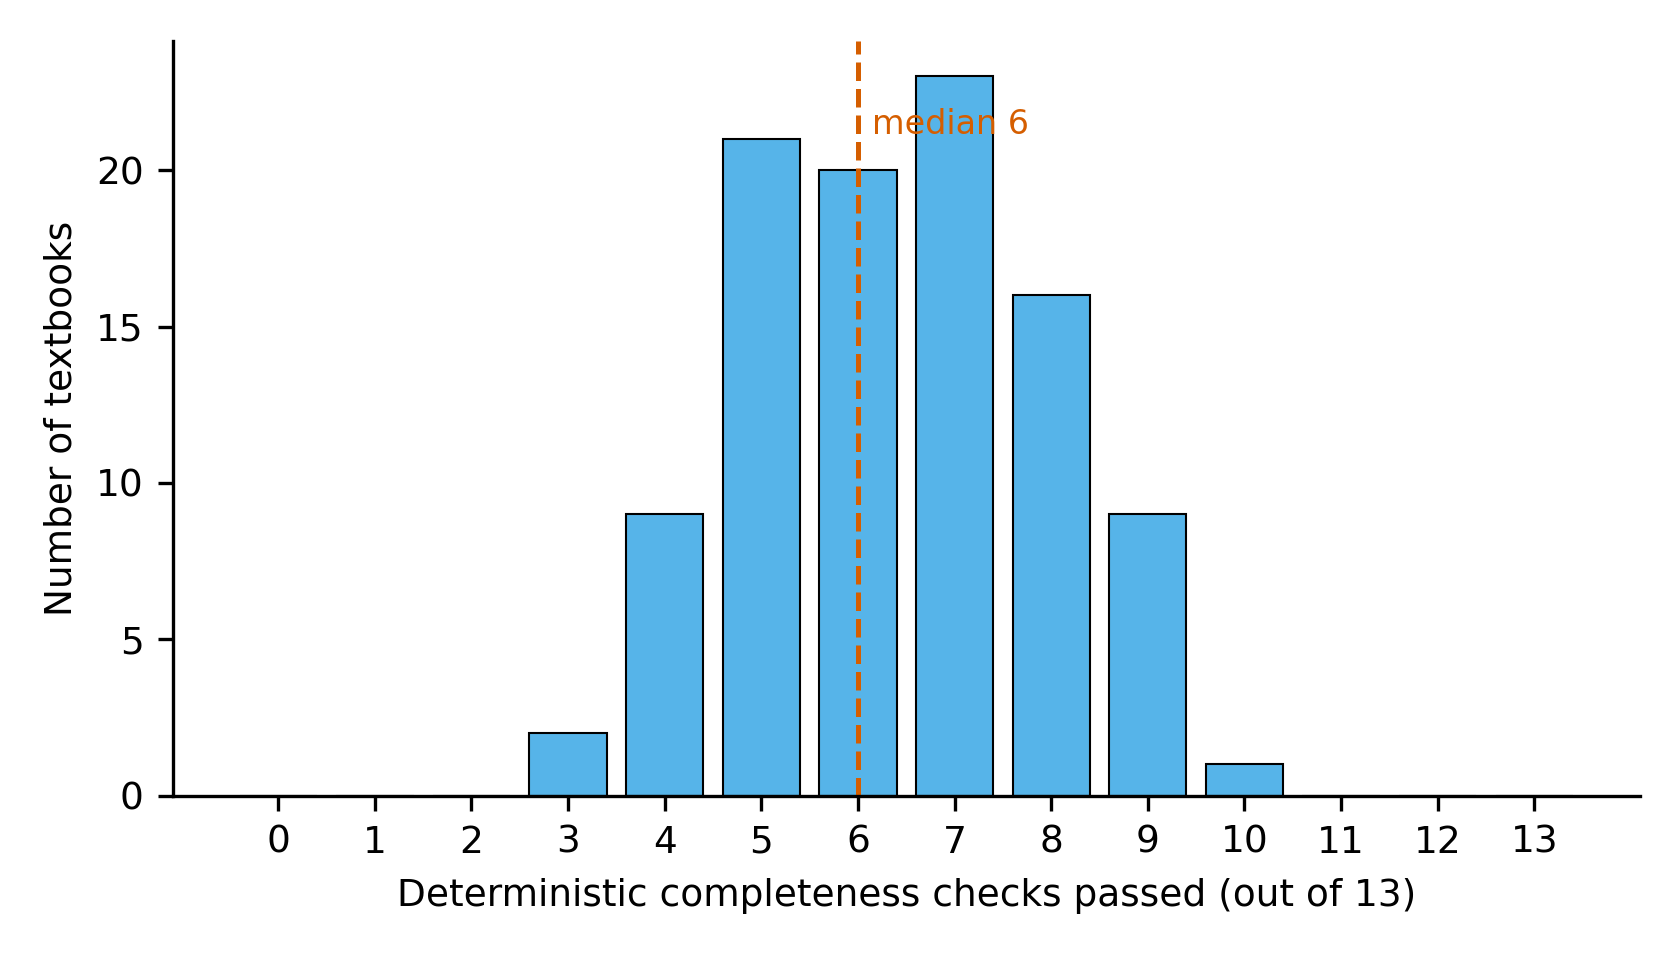
\includegraphics[width=0.78\textwidth]{figures/census-histogram.png}
  \caption{Distribution of the number of scripted completeness checks passed (out of 13) across 101 MkDocs book projects in one author's workspace. The distribution is centered near six, with a long tail of books passing few checks; only one book passes ten and none passes more. The dashed line marks the median.}
  \label{fig:census}
\end{figure}
